\documentclass[11pt,a4paper]{article}
\usepackage{creh-article}
\usepackage{float}
\begin{document}
\ArticleTitle{INVESTIGACIÓN / APRENDIZAJE AUTOMÁTICO}{Algoritmos de ML para reconocer el alfabeto estático de la lengua de señas peruana}{13 de octubre de 2026}
\ArticleAbstract{Se estudia un sistema de reconocimiento de letras estáticas que transforma 21 puntos de la mano en 15 ángulos articulares y una orientación planar. La comparación emplea 2500 registros de geometría manual, 16 características y 25 clases balanceadas: 24 letras y espacio. Se entrenan y comparan seis algoritmos de aprendizaje automático: árbol de decisión, Extra Trees, KNN, regresión logística, Random Forest y SVM radial. La evaluación empleó 2000 registros de entrenamiento, validación cruzada de cinco particiones exclusivamente dentro de ese conjunto y 500 registros de prueba reservados. Extra Trees alcanzó 97,80\% de exactitud y 97,78\% de F1 macro; al conservar el orden por clase y reservar sus últimos 20 registros, alcanzó 96,20\%. Todos los clasificadores se entrenaron localmente en CPU, sin contratar GPU. La tabla no contiene identidades de participantes ni sesiones: los resultados describen este dataset y no acreditan generalización a personas nuevas, condiciones de cámara distintas o lengua de señas continua.}
\Keywords{lengua de señas peruana; aprendizaje automático; MediaPipe; clasificación estática; reproducibilidad.}

\section{Introducción y alcance}
La comunicación mediante lengua de señas involucra configuraciones manuales, movimiento, expresión y contexto. Este trabajo aborda una tarea más limitada: clasificar letras estáticas del alfabeto dactilológico a partir de la geometría de una sola mano. Concatenar letras reconocidas permite componer texto, pero no constituye traducción de la gramática de la lengua de señas.

El reconocimiento de configuraciones manuales puede organizarse en dos etapas: extracción de características geométricas y clasificación supervisada. MediaPipe permite localizar puntos de la mano a partir de imágenes RGB mediante modelos previamente entrenados \cite{zhang}. Sobre esa representación pueden entrenarse distintos algoritmos de ML clásico sin entrenar de nuevo el detector ni requerir una GPU.

El objetivo de este estudio es entrenar y comparar seis clasificadores bajo un mismo conjunto de características y particiones comunes, para determinar cuál obtiene el mejor desempeño observado. Se evalúan árbol de decisión, Extra Trees, KNN, regresión logística, Random Forest y SVM radial. La comparación considera exactitud, medidas macro, MCC y coste computacional, sin presuponer un ganador. Este documento presenta los resultados de un experimento reproducible realizado en CREH Labs y se publica como preprint, sin revisión por pares declarada.

\section{Adquisición de imágenes y preparación de los datos}
\subsection{Captura y recorte de la mano}
La adquisición comienza al encender la cámara y asignar la letra que representa la postura de la mano. MediaPipe localiza 21 puntos: la muñeca y las articulaciones de los cinco dedos. Los valores mínimos y máximos de sus coordenadas horizontales y verticales delimitan un rectángulo que contiene los puntos detectados. Las coordenadas normalizadas se convierten a píxeles multiplicándolas por el ancho y el alto del cuadro.

Para conservar contexto alrededor de la mano se toma como referencia el mayor lado del rectángulo, $d=\max(x_{\max}-x_{\min},y_{\max}-y_{\min})$. La rutina original recuperada añade un margen de $0{,}25d$ y define los límites del recorte como
\begin{align}
x'_0&=\max(x_{\min}-\lfloor0{,}25d\rfloor,0), &
x'_1&=\min(x_{\min}+\lfloor1{,}25d\rfloor,W),\\
y'_0&=\max(y_{\min}-\lfloor0{,}25d\rfloor,0), &
y'_1&=\min(y_{\min}+\lfloor1{,}25d\rfloor,H).
\end{align}
Aquí $W$ y $H$ son las dimensiones del cuadro. El recorte se ancla en los mínimos del rectángulo; antes de limitarlo al borde de la imagen, cada lado mide aproximadamente $1{,}5d$. Esta construcción utiliza un 25\% del lado de referencia como margen. Cuando la mano llega al borde del cuadro, el recorte queda limitado por la imagen disponible.

Solo se guardan recortes cuyo ancho y alto superan 224 píxeles. Los aceptados se redimensionan a $224\times224$ píxeles, de modo que las imágenes tengan una resolución común. El redimensionamiento directo puede modificar la relación de aspecto si el recorte quedó truncado. Cada imagen se asocia a su letra, y la rutina intenta reunir 100 imágenes por etiqueta. Este procedimiento describe el código histórico de adquisición; las métricas de este estudio corresponden a la tabla de características disponible y no a una nueva campaña de captura. No se ha verificado una correspondencia imagen por imagen entre ese archivo y los registros evaluados.

\subsection{De imágenes a características geométricas}
Las imágenes representan la apariencia de una postura manual. Los puntos de la mano describen su estructura; de ellos se derivan 15 ángulos articulares y una orientación global. La tabla angular almacena esas 16 medidas junto con la clase de la seña, en lugar de entregar los píxeles directamente al clasificador. Esta representación compacta permite comparar algoritmos de aprendizaje automático con el mismo tipo de entrada.

El conjunto evaluado contiene 2500 registros, 100 por clase. Se verificó la ausencia de valores no finitos y de duplicados exactos. Los ángulos articulares están entre 0 y 180 grados; la orientación está entre 0 y 360 grados, excluyendo 360. Cada registro describe una configuración de la mano y su etiqueta. La copia archivada en Kaggle se cita como fuente de acceso a los datos \cite{dataset}; su ubicación informática no sustituye la descripción del proceso de adquisición.

Las 25 clases son A, B, C, D, E, F, G, H, I, K, L, M, N, O, P, Q, R, S, T, U, V, W, X e Y, más espacio. J, Ñ y Z no forman parte de las clases evaluadas. La clase espacio permite separar palabras. Las ilustraciones adicionales de la interfaz funcionan como referencias de aprendizaje.

\section{Representación geométrica y algoritmos de clasificación}
\subsection{Localización de la mano}
En ejecución, un cuadro RGB se entrega a MediaPipe Hand Landmarker. El detector localiza la palma y el estimador proporciona 21 puntos normalizados $p_i=(x_i,y_i,z_i)$: muñeca ($i=0$) y cuatro articulaciones por dedo. El sistema trabaja con una mano y umbrales de detección, presencia y seguimiento de 0,5. Si no se detecta mano, se elimina el historial temporal y no se emite una letra. Estos pasos son parte de la aplicación; el entrenamiento actual comienza directamente desde los ángulos almacenados, sin volver a procesar imágenes.

\subsection{Extracción de las 16 características}
Se consideran los índices
\[
\mathcal I=\{1,2,3,5,6,7,9,10,11,13,14,15,17,18,19\}.
\]
Para cada $i\in\mathcal I$, el punto anterior es $q_i=p_0$ cuando $i\in\{5,9,13,17\}$, y $q_i=p_{i-1}$ en otro caso. Se calculan
\begin{equation}
a_i=\|q_i-p_{i+1}\|_2,\quad b_i=\|q_i-p_i\|_2,\quad c_i=\|p_{i+1}-p_i\|_2.
\end{equation}
La ley de cosenos produce el ángulo interior en $p_i$:
\begin{equation}
\theta_i=\operatorname{round}_{\mathrm{par}}\left(\frac{180}{\pi}\arccos\left(\frac{b_i^2+c_i^2-a_i^2}{2b_ic_i}\right)\right).
\end{equation}
El redondeo al par conserva la convención de Python. La rutina de extracción solo calcula $\arccos$ cuando el coseno está estrictamente entre $-1$ y $1$; fuera de ese intervalo fija el ángulo en cero. Si alguna distancia es cero, puede faltar una característica: un cuadro que no produzca exactamente 16 valores se descarta. Los cuadros degenerados requieren tratamiento explícito; en este estudio se utiliza la tabla angular ya disponible.

La orientación de muñeca a base del dedo medio se calcula como
\begin{equation}
\phi=\frac{180}{\pi}\operatorname{atan2}(y_0-y_9,x_9-x_0),\qquad
\phi\leftarrow\phi+360\ \text{si }\phi<0.
\end{equation}
No se redondea $\phi$. El vector final concatena los 15 $\theta_i$ en el orden de las columnas y $\phi$. La posición absoluta desaparece al usar diferencias y distancias; la orientación se mantiene de manera explícita. La codificación lineal de $\phi$ introduce una discontinuidad entre 359 y 0 grados; no se sustituye por seno y coseno porque ello cambiaría el contrato de 16 entradas.

\subsection{Algoritmos de aprendizaje automático}
Los seis modelos reciben el mismo vector de 16 características y predicen una de las 25 clases. Cada familia tiene una regla de aprendizaje diferente; los parámetros utilizados se detallan en la metodología.

\paragraph{Árbol de decisión.} Divide recursivamente el espacio de atributos mediante umbrales que reducen la impureza Gini, $G=1-\sum_k p_k^2$. La predicción se obtiene de la clase mayoritaria de la hoja alcanzada. Un árbol individual ofrece inferencia sencilla, pero sus divisiones pueden ser sensibles a variaciones de los datos.

\paragraph{Extra Trees.} Construye un ensamble con selección aleatoria de atributos y puntos de corte \cite{geurts}. En cada nodo compara divisiones aleatorias por su reducción de impureza. Los árboles usan el conjunto de entrenamiento sin remuestreo bootstrap. La predicción agrega sus distribuciones de clase; la aleatorización busca reducir la dependencia entre árboles.

\paragraph{KNN.} Conserva ejemplos de entrenamiento y clasifica cada consulta mediante los cinco vecinos más cercanos en distancia euclídea. Su regla depende de la escala de los atributos, por lo que se estandarizan las características dentro de cada partición de entrenamiento.

\paragraph{Regresión logística.} Aprende funciones lineales para las clases mediante minimización de la pérdida logística con regularización. Para clase $k$, el modelo multiclase utiliza
\begin{equation}
P(y=k\mid x)=\frac{\exp(w_k^\top x+b_k)}{\sum_j\exp(w_j^\top x+b_j)}.
\end{equation}
La estandarización facilita la optimización. Sus fronteras lineales pueden limitar la representación de configuraciones complejas.

\paragraph{Random Forest.} Combina árboles entrenados sobre muestras bootstrap y considera subconjuntos aleatorios de atributos al buscar divisiones. A diferencia de Extra Trees, busca cortes de mejor impureza entre los valores disponibles. Ambos ensambles promedian las distribuciones de sus hojas:
\begin{equation}
\widehat P(y=k\mid x)=\frac1T\sum_{t=1}^{T}P_t(y=k\mid x),\qquad
\widehat y=\arg\max_k\widehat P(y=k\mid x).
\end{equation}
En este estudio se fija $T=100$ para ambas familias. Scikit-learn convierte las entradas a float32 al recorrer los árboles \cite{sklearn}.

\paragraph{SVM radial.} Busca fronteras de margen amplio en un espacio inducido por el kernel $K(x,x')=\exp(-\gamma\|x-x'\|_2^2)$. Los parámetros $C$ y $\gamma$ controlan regularización y alcance de la similitud. Se usa estandarización y no se activa estimación de probabilidades.

Las medidas de confianza de los modelos, cuando están disponibles, no equivalen a su exactitud global ni se consideran probabilidades calibradas de acierto.

\subsection{Estabilización, mensaje y voz}
La aplicación mantiene una ventana de ocho predicciones. Una clase se confirma cuando obtiene al menos seis votos y la confianza media de sus votos alcanza 0,45. La confirmación temporal no se utilizó para calcular las métricas del CSV, porque este no incluye secuencias o tiempos. Una letra confirmada se añade al mensaje cuando cambia respecto de la última emitida. Retirar la mano restablece ese estado y permite repetir una letra; espacio separa palabras. El mensaje puede editarse, copiarse y leerse mediante las voces del dispositivo. Estas operaciones posteriores no cambian los árboles ni constituyen corrección lingüística automática.

\section{Diseño experimental}
\subsection{Particiones y prevención de contaminación}
Se fijó antes de la comparación una partición aleatoria estratificada 80/20, con semilla 42: 2000 registros para entrenamiento y 500 para prueba, 20 de prueba por clase. Se aplicó validación cruzada estratificada de cinco particiones solo a los 2000 registros de entrenamiento \cite{cv}. Cada ajuste interno empleó 1600 registros y validó con 400. No hubo búsqueda de hiperparámetros sobre el conjunto de prueba.

Como comprobación de sensibilidad al orden, se reservan los últimos 20 registros de cada clase y se entrena con sus primeros 80. Esta segunda partición preserva el orden de filas de origen, pero no se interpreta como evaluación temporal o entre personas: esas identidades no están documentadas. Los modelos de esa prueba se ajustan de nuevo, sin reutilizar el modelo de la partición aleatoria.

\subsection{Modelos comparados}
Random Forest utiliza 100 árboles, \texttt{max\_features=sqrt} y bootstrap estándar. El árbol de decisión usa criterio Gini sin límite de profundidad. KNN emplea cinco vecinos y distancia euclídea. SVM usa kernel radial, $C=1$ y \texttt{gamma=scale}. La regresión logística usa $C=1$ y hasta 3000 iteraciones. KNN, SVM y regresión logística se incluyen en pipelines con \texttt{StandardScaler}, ajustado dentro de cada conjunto de entrenamiento y de cada partición de validación. Los árboles reciben las características sin escalado. Todos los parámetros estocásticos pertinentes usan semilla 42. No se afirma que estas configuraciones sean óptimas para cada familia.

\subsection{Métricas, incertidumbre y coste}
Se informa exactitud, precisión macro, recall macro, F1 macro y coeficiente de correlación de Matthews (MCC). Las medidas macro promedian por igual las 25 clases; en este conjunto balanceado, recall macro coincide con exactitud. La exactitud es la proporción de predicciones correctas. Para cada clase, precisión es $TP/(TP+FP)$, recall es $TP/(TP+FN)$ y F1 es su media armónica. Los indicadores se calculan sobre los 500 registros reservados, sin aplicar un umbral de abstención.

Para Extra Trees se obtuvo un intervalo percentil bootstrap del 95\% con 10000 remuestreos de los aciertos de prueba y semilla 42. Ese intervalo supone unidades intercambiables y puede ser optimista si las filas son cuadros correlacionados. No reemplaza una evaluación por personas. No se reporta AUC uniforme porque SVM se entrenó sin probabilidades y no se añadió una calibración que alterara la comparación.

El tiempo de ajuste es de un entrenamiento con 2000 filas y no incluye validación cruzada. La inferencia se midió después de un calentamiento, promediando diez lotes de 500 registros y dividiendo por el tamaño del lote. No incluye cámara, MediaPipe, transmisión al trabajador, dibujo ni voz; por tanto, no es latencia de usuario ni FPS de la aplicación. Se ejecutó en Linux, con dos CPU lógicas disponibles, un hilo por estimador y límites de un hilo para las bibliotecas numéricas. Los tiempos son medidas de esta ejecución en un entorno compartido.

\section{Resultados}
\begin{table}[ht]
\centering\small
\caption{Resultados en 500 registros reservados. Exactitud, precisión, recall y F1 se expresan en porcentaje.}
\resizebox{\linewidth}{!}{\begin{tabular}{lrrrrr}\toprule
Modelo & Exactitud & Prec. macro & Recall macro & F1 macro & MCC\\\midrule
Árbol de decisión & 93.40 & 93.65 & 93.40 & 93.36 & 0.9314 \\
Extra Trees & 97.80 & 98.06 & 97.80 & 97.78 & 0.9772 \\
KNN & 96.20 & 96.44 & 96.20 & 96.17 & 0.9605 \\
Regresión logística & 96.60 & 97.15 & 96.60 & 96.53 & 0.9649 \\
Random Forest & 96.80 & 97.06 & 96.80 & 96.70 & 0.9668 \\
SVM RBF & 96.80 & 97.16 & 96.80 & 96.79 & 0.9668 \\
\bottomrule\end{tabular}}
\end{table}
Extra Trees acertó 489 de 500 registros y obtuvo F1 macro de 97,78\%. El intervalo bootstrap del 95\% para exactitud fue [96.40\%, 99.00\%]. Su promedio de exactitud en validación cruzada fue 97,65\%, con desviación estándar de 0,34 puntos porcentuales. Random Forest y SVM obtuvieron 96,80\% en prueba; la regresión logística, 96,60\%; KNN, 96,20\%; y el árbol individual, 93,40\%.

\begin{table}[ht]
\centering\small
\caption{Validación cruzada (media $\pm$ desviación estándar, en porcentaje), prueba con orden conservado y costes observados.}
\resizebox{\linewidth}{!}{\begin{tabular}{lrrrr}\toprule
Modelo & CV exactitud & Orden: exactitud & Ajuste (s) & Lote (ms/registro)\\\midrule
Árbol de decisión & 94.60 $\pm$ 0.88 & 88.40 & 0.048 & 0.0009 \\
Extra Trees & 97.65 $\pm$ 0.34 & 96.20 & 3.417 & 0.5102 \\
KNN & 95.90 $\pm$ 0.42 & 93.80 & 0.009 & 0.0327 \\
Regresión logística & 95.60 $\pm$ 1.05 & 93.00 & 0.143 & 0.0015 \\
Random Forest & 97.20 $\pm$ 0.45 & 95.20 & 0.976 & 0.0964 \\
SVM RBF & 96.25 $\pm$ 0.64 & 95.00 & 0.077 & 0.0972 \\
\bottomrule\end{tabular}}
\end{table}
\begin{figure}[ht]
\centering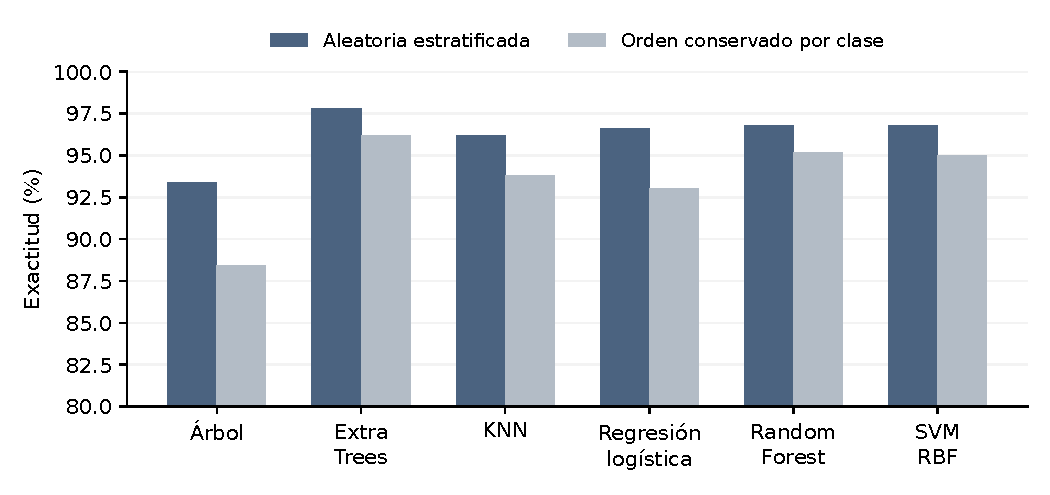
\includegraphics[width=.88\linewidth]{comparison.pdf}
\caption{Comparación de las dos particiones. Ambos protocolos usan 500 registros de prueba; ninguno separa identidades de participantes.}
\end{figure}
La partición por orden reduce la exactitud de todos los métodos. Extra Trees conserva el mayor valor observado, 96,20\%, mientras que el árbol individual baja a 88,40\%. Este contraste indica sensibilidad a cómo se separan los registros, sin demostrar una causa temporal específica. No se realizaron pruebas de superioridad estadística entre pares, y las diferencias pequeñas no justifican afirmar una ventaja universal.

\begin{figure}[ht]
\centering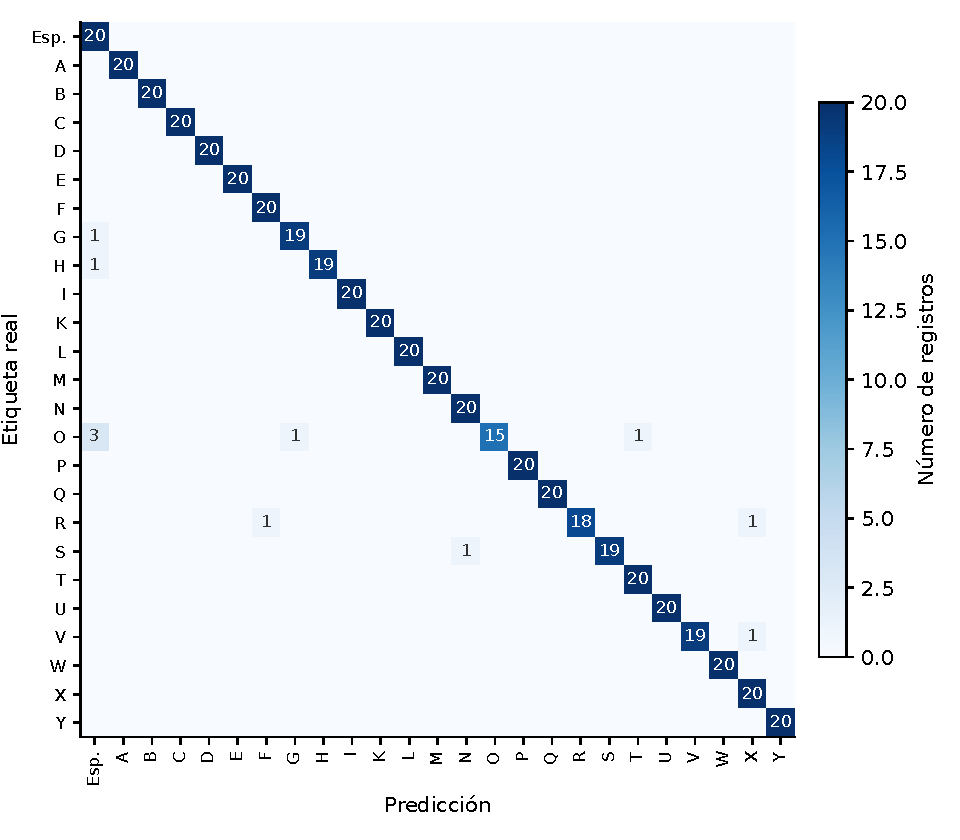
\includegraphics[width=.85\linewidth]{confusion.pdf}
\caption{Matriz de confusión de Extra Trees en la prueba aleatoria. Cada fila tiene 20 registros; ``Esp.'' es espacio. Los números corresponden a conteos, no porcentajes.}
\end{figure}

\section{Selección del algoritmo a partir de los resultados}
La elección se realiza a partir de las métricas comparativas y no se plantea como una premisa del estudio. Extra Trees presenta los mayores valores observados de exactitud y F1 macro tanto en la partición aleatoria como en la prueba que conserva el orden por clase. Por ello se selecciona como alternativa de reconocimiento para el dataset estudiado, manteniendo las restricciones de generalización descritas.

Después de la evaluación se ajustó el algoritmo seleccionado con las 2500 filas para disponer de un artefacto de uso. Este ajuste incluye las filas antes reservadas y no constituye una nueva evaluación independiente. Los puntajes de las tablas corresponden a los modelos entrenados con 2000 registros.

El clasificador seleccionado se exportó a un formato binario de 16 entradas y 25 etiquetas para una posible integración en web y Android. El lector web reprodujo las probabilidades y etiquetas de Python en 400 vectores sintéticos, con tolerancia de $10^{-6}$ para probabilidades. Esa comprobación valida la implementación del lector; no equivale a evaluar 400 imágenes o personas. La integración de un modelo y la validación de cámara constituyen tareas posteriores al experimento comparativo.

\section{Discusión y límites}
La representación angular compacta permite comparar clasificadores clásicos sin entrenamiento de redes profundas. Extra Trees fue el mejor método observado en exactitud y F1 bajo las dos particiones, pero su tiempo de inferencia por lote fue mayor que el de otros modelos en esta ejecución. La regresión logística y el árbol individual muestran un coste reducido, aunque sacrifican exactitud; la elección de interfaz debe considerar tanto reconocimiento como latencia total.

El dataset es pequeño, balanceado y sin metadatos de participantes. Ausencia de duplicados exactos no implica independencia entre registros: cuadros consecutivos o manos de una misma persona pueden ser muy parecidos. La validación cruzada aleatoria tampoco corrige esa dependencia. La prueba de orden ofrece una comprobación adicional, pero no equivale a dejar fuera una persona o una sesión.

La correspondencia entre características del CSV y puntos extraídos en una cámara nueva debe comprobarse empíricamente. Normalizar coordenadas por ancho y alto, cambiar la relación de aspecto, reflejar la imagen o modificar el detector puede alterar ángulos y orientación. Este estudio no evaluó imágenes originales ni adquisición en vivo; no permite cuantificar precisión por dispositivo, mano dominante, iluminación, distancia o condiciones de oclusión. Tampoco valida señas dinámicas, varias manos, expresiones faciales ni vocabulario completo.

Como pasos posteriores se requieren una prueba con personas y sesiones independientes, protocolos de cámara documentados, una política de abstención por baja confianza y, si se modifica la orientación o el tratamiento de ángulos degenerados, una nueva versión del esquema de características. La extracción de puntos y el clasificador deben mantenerse sincronizados.

\section{Conclusiones}
Se entrenaron y compararon seis algoritmos de aprendizaje automático en CPU con 2500 registros, 16 características geométricas y 25 clases balanceadas. La representación compartida y las particiones comunes permitieron contrastar exactitud, F1 macro, MCC y coste de procesamiento bajo el mismo protocolo.

Los resultados muestran que \textbf{Extra Trees fue el mejor algoritmo de los evaluados para este dataset}: obtuvo 97,80\% de exactitud y 97,78\% de F1 macro en la prueba aleatoria, y 96,20\% de exactitud en la prueba por orden. Esa conclusión se deriva de los experimentos y está acotada a sus datos y configuraciones; no demuestra superioridad universal ni generalización a personas nuevas. El entrenamiento de los clasificadores no requirió GPU.

\section*{Material complementario}
El código de captura recuperado del notebook histórico se ofrece como material complementario en la ficha web de este artículo. Permite examinar el cálculo de los límites, el margen de 25\% y la resolución de $224\times224$ píxeles. Se conserva como evidencia del procedimiento original; no se ejecutó la cámara durante la comparación. La aplicación existente está disponible en \url{https://senas.crehlabs.com}. Los materiales del experimento incluyen las configuraciones de los seis clasificadores, las particiones comunes y las métricas de evaluación.

\begin{thebibliography}{9}
\bibitem{geurts} P. Geurts, D. Ernst y L. Wehenkel. Extremely randomized trees. \emph{Machine Learning}, 63:3--42, 2006. \url{https://doi.org/10.1007/s10994-006-6226-1}.
\bibitem{zhang} F. Zhang, V. Bazarevsky, A. Vakunov, A. Tkachenka, G. Sung, C.-L. Chang y M. Grundmann. MediaPipe Hands: On-device Real-time Hand Tracking. arXiv:2006.10214, 2020. \url{https://arxiv.org/abs/2006.10214}.
\bibitem{dataset} Cristhian Egoavil. CSV angles static. Dataset de Kaggle, consultado el 13 de octubre de 2026. \url{https://www.kaggle.com/datasets/cristhianegoavil/csv-angles-static}.
\bibitem{sklearn} Scikit-learn developers. ExtraTreesClassifier: documentación de referencia. \url{https://scikit-learn.org/stable/modules/generated/sklearn.ensemble.ExtraTreesClassifier.html}. Biblioteca utilizada: scikit-learn 1.9.0.
\bibitem{cv} Scikit-learn developers. Cross-validation: evaluating estimator performance. \url{https://scikit-learn.org/stable/modules/cross_validation.html}.
\end{thebibliography}
\end{document}
